%====================================================================%
%                  MORIOND.TEX                                       %
% This latex file rewritten from various sources for use in the      %
% preparation of the standard proceedings Volume, latest version     %
% for the Neutrino'96 Helsinki conference proceedings                %
% by Susan Hezlet with acknowledgments to Lukas Nellen.              %
% Some changes are due to David Cassel.                              %
%====================================================================%

%\documentstyle[11pt,moriond,epsfig]{article}
\documentclass[11pt]{article}
\usepackage{moriond,epsfig}


\bibliographystyle{unsrt}    
% for BibTeX - sorted numerical labels by order of
% first citation.

% A useful Journal macro
\def\Journal#1#2#3#4{{#1} {\bf #2}, #3 (#4)}

% Some useful journal names
\def\NCA{\em Nuovo Cimento}
\def\NIM{\em Nucl. Instrum. Methods}
\def\NIMA{{\em Nucl. Instrum. Methods} A}
\def\NPB{{\em Nucl. Phys.} B}
\def\PLB{{\em Phys. Lett.}  B}
\def\PRL{\em Phys. Rev. Lett.}
\def\PRD{{\em Phys. Rev.} D}
\def\ZPC{{\em Z. Phys.} C}

% Some other macros used in the sample text
\def\st{\scriptstyle}
\def\sst{\scriptscriptstyle}
\def\mco{\multicolumn}
\def\epp{\epsilon^{\prime}}
\def\vep{\varepsilon}
\def\ra{\rightarrow}
\def\ppg{\pi^+\pi^-\gamma}
\def\vp{{\bf p}}
\def\ko{K^0}
\def\kb{\bar{K^0}}
\def\al{\alpha}
\def\ab{\bar{\alpha}}
\def\be{\begin{equation}}
\def\ee{\end{equation}}
\def\bea{\begin{eqnarray}}
\def\eea{\end{eqnarray}}
\def\CPbar{\hbox{{\rm CP}\hskip-1.80em{/}}}
%temp replacement due to no font

\def \GeVmass {GeV\xspace}
\def \GeVmom {GeV\xspace}
\def \sqrts {$\sqrt{s}=7$~TeV\xspace}
\def \etmiss {\ensuremath{E_{\mathrm{T}}\hspace{-1.1em}/\kern0.5em}\xspace}
\def \pt{\ensuremath{p_{\rm T}}\xspace}
\def \pp {proton-proton\xspace}

%%%%%%%%%%%%%%%%%%%%%%%%%%%%%%%%%%%%%%%%%%%%%%%%%%
%                                                %
%    BEGINNING OF TEXT                           %
%                                                %
%%%%%%%%%%%%%%%%%%%%%%%%%%%%%%%%%%%%%%%%%%%%%%%%%%
\begin{document}
\vspace*{4cm}
\title{EXOTICA SEARCHES AT THE CMS EXPERIMENT}

\author{F. SANTANASTASIO \\(ON BEHALF OF THE CMS COLLABORATION)}

\address{University of Maryland, Department of Physics - John S. Toll Physics Building, \\ College Park, MD 20742-4111, United States of America}

\maketitle\abstracts{
This paper presents the results of searches for various new physics 
phenomena in proton-proton collisions at $\sqrt{s}=7$~TeV delivered 
by the LHC and collected with the CMS detector in 2010. 
While the sensitivity of these early searches varies, 
in many cases they set the most stringent limits on these 
new physics phenomena. These results demonstrate good understanding 
of the detector and backgrounds in a variety of channels, 
which is a fundamental component of successful searches in view 
of the much larger data sample expected to be delivered by LHC in 2011 and beyond.
%% This is where the abstract should be placed. It should consist of one paragraph
%% and give a concise summary of the material in the article below.
%% Replace the title, authors, and addresses within the curly brackets
%% with your own title, authors, and addresses; please use
%% capital letters for the title and the authors. You may have as many authors and
%% addresses as you wish. It's preferable not to use footnotes in the abstract
%% or the title; the
%% acknowledgments for funding bodies etc. are placed in a separate section at
%% the end of the text.
}

\section{Section}
\subsection{SubSection}\label{subsec:test}


\begin{table}[htbp]
\caption{CAPTION}
\vspace{0.4cm}
\begin{center}
\begin{tabular}{|c|c|c|}
\hline
& & \\
& & \\ 
\hline
\end{tabular}
\end{center}
\end{table}

\begin{figure}[htbp]
%\vskip 2.5cm
  \begin{center}
    \begin{tabular}{cc}
      \psfig{figure=beta_vs_m_excl_comb.ps,height=3in} &
      \psfig{figure=beta_vs_m_excl_comb.ps,height=3in} \\
%      \resizebox{7.9cm}{!}{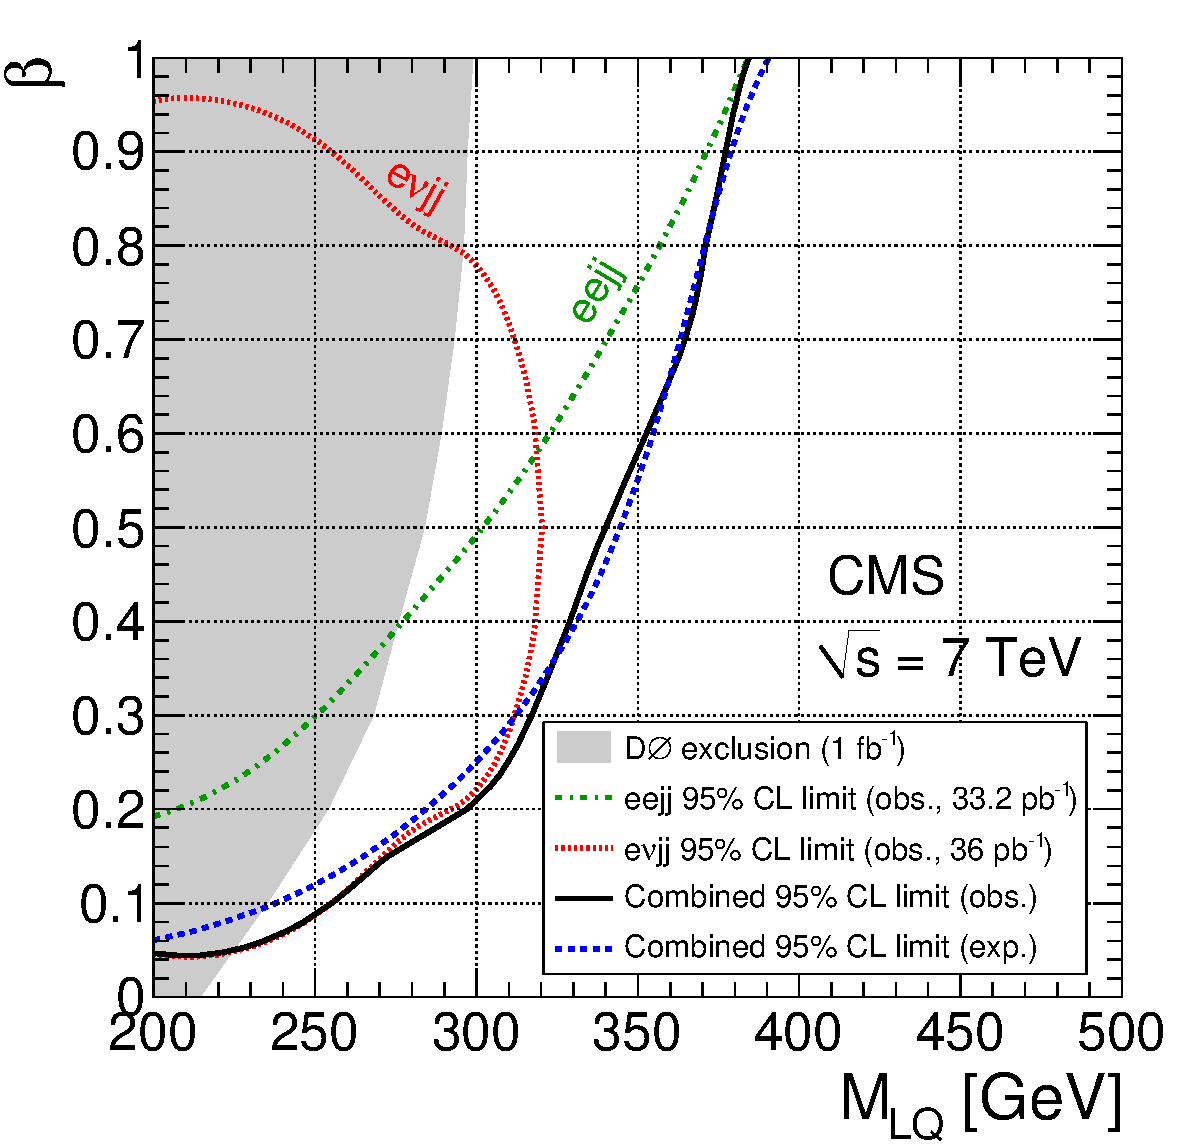
\includegraphics[angle=0]{beta_vs_m_excl_comb.pdf}} &
%      \resizebox{7.9cm}{!}{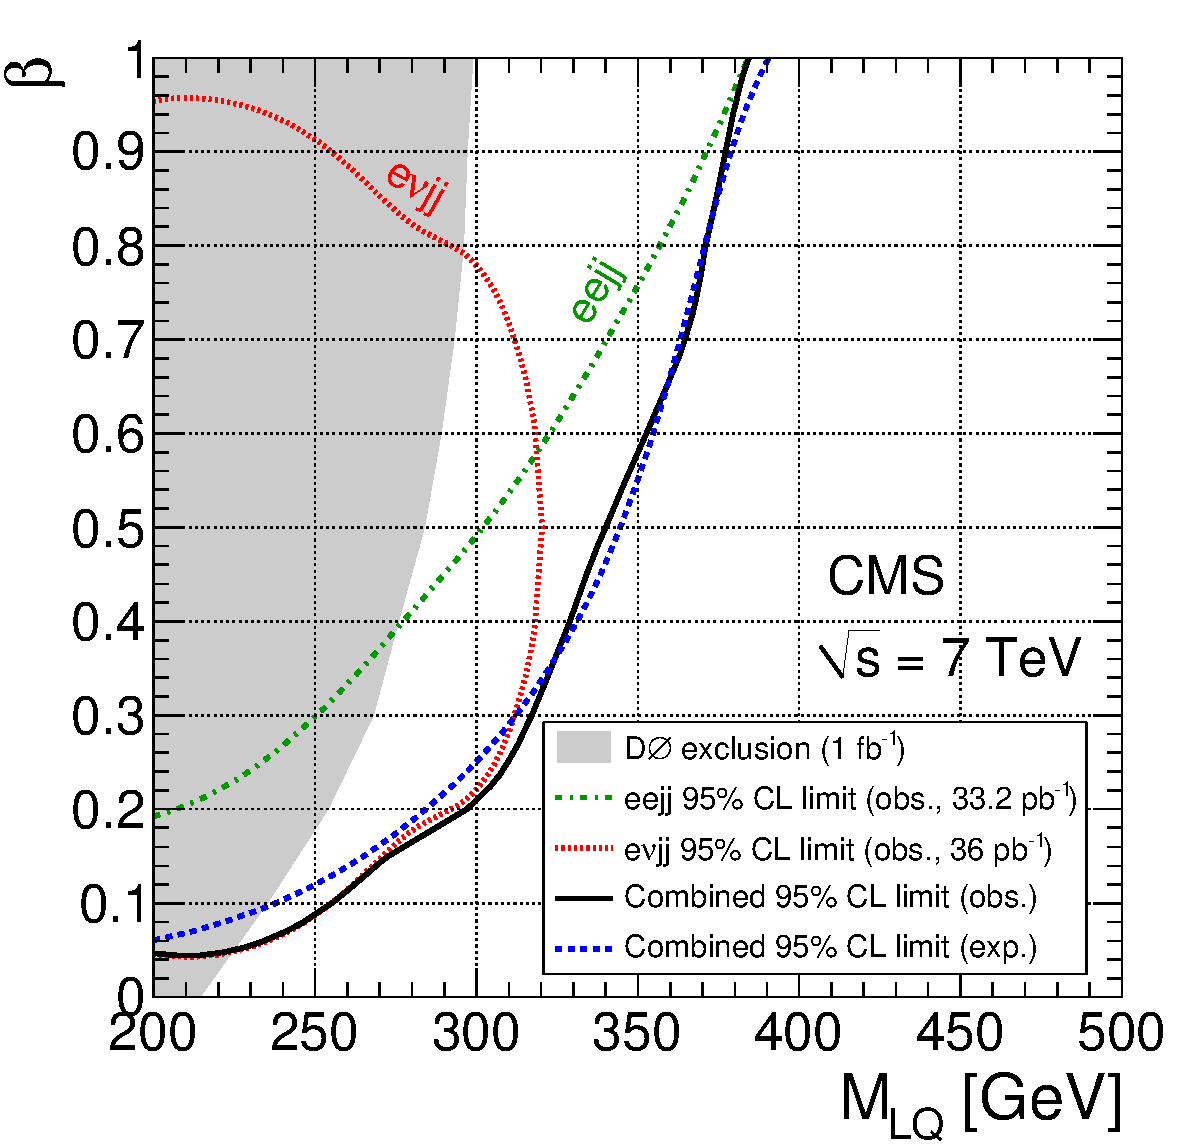
\includegraphics[angle=0]{beta_vs_m_excl_comb.pdf}} \\
    \end{tabular}
    \caption{CAPTION}
    \label{fig:AfterPresel}
  \end{center}
\end{figure}

\section*{Acknowledgments}

\section*{References}
\begin{thebibliography}{99}

\bibitem{ja}C Jarlskog in {\em CP Violation}, ed. C Jarlskog
(World Scientific, Singapore, 1988).

\bibitem{ma}L. Maiani, \Journal{\PLB}{62}{183}{1976}.

\bibitem{bu}J.D. Bjorken and I. Dunietz, \Journal{\PRD}{36}{2109}{1987}.

\bibitem{bd}C.D. Buchanan {\it et al}, \Journal{\PRD}{45}{4088}{1992}.

\end{thebibliography}

\end{document}

%%%%%%%%%%%%%%%%%%%%%%
% End of moriond.tex  %
%%%%%%%%%%%%%%%%%%%%%%

